\documentclass[tikz,border=15pt]{standalone}
\usepackage{amsmath,amssymb}
\usetikzlibrary{arrows.meta}

\begin{document}
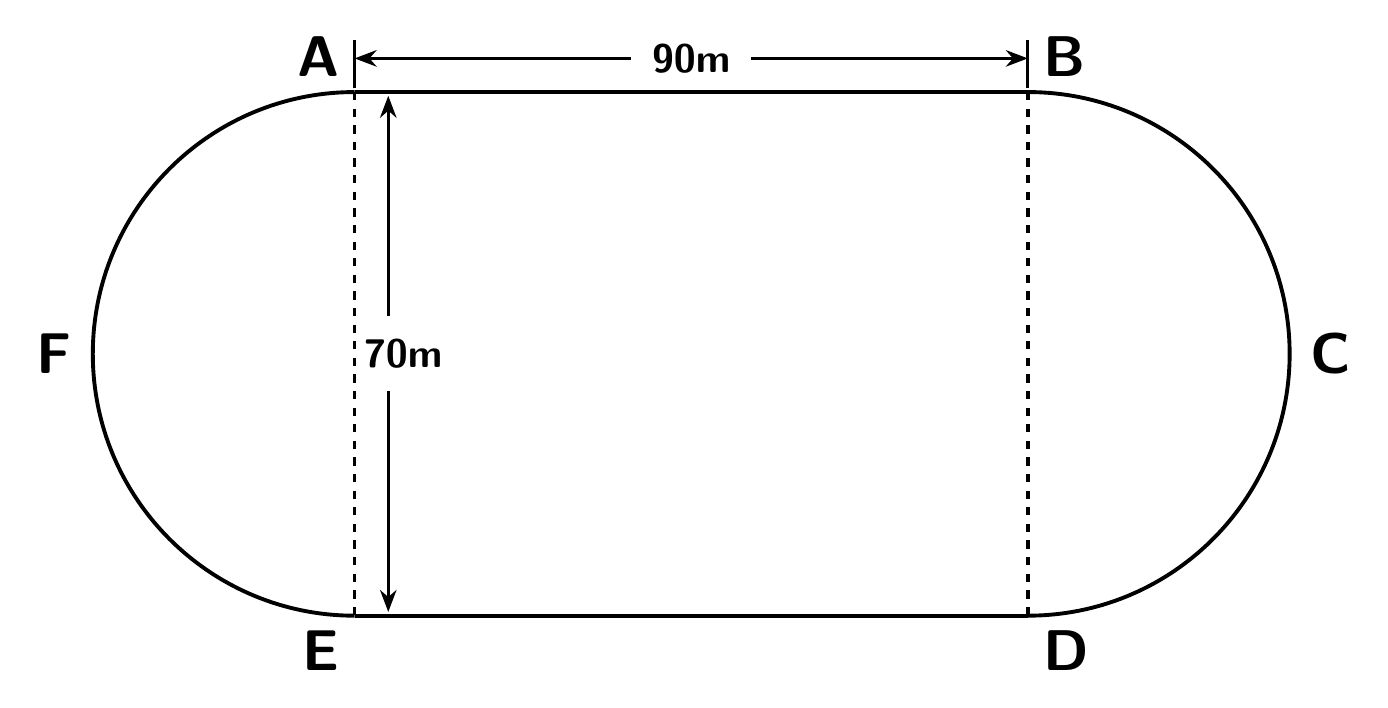
\begin{tikzpicture}[>=Stealth, scale=0.95]
    % Running track: AB = 9.0 cm, diameter AE = 7.0 cm (radius R = 3.5 cm)
    \def\w{4.5} % half width, so AB = 9.0
    \def\r{3.5} % radius, so height = 7.0
    
    \coordinate (A) at (-\w, \r);
    \coordinate (B) at (\w, \r);
    \coordinate (D) at (\w, -\r);
    \coordinate (E) at (-\w, -\r);
    \coordinate (F) at ({-\w - \r}, 0);
    \coordinate (C) at ({\w + \r}, 0);
    
    % Outer boundary of running track
    \draw[line width=1.4pt] (A) -- (B);
    \draw[line width=1.4pt] (E) -- (D);
    \draw[line width=1.4pt] (D) arc (-90:90:\r);
    \draw[line width=1.4pt] (A) arc (90:270:\r);
    
    % Dashed internal divider lines
    \draw[line width=1.2pt, dashed] (A) -- (E);
    \draw[line width=1.2pt, dashed] (B) -- (D);
    
    % Vertices labels in bold sans-serif
    \node[above left=2pt, font=\huge\sffamily\bfseries] at (A) {A};
    \node[above right=2pt, font=\huge\sffamily\bfseries] at (B) {B};
    \node[right=4pt, font=\huge\sffamily\bfseries] at (C) {C};
    \node[below right=2pt, font=\huge\sffamily\bfseries] at (D) {D};
    \node[below left=2pt, font=\huge\sffamily\bfseries] at (E) {E};
    \node[left=4pt, font=\huge\sffamily\bfseries] at (F) {F};
    
    % Dimension callout for AB = 90m (above top line)
    \draw[line width=1.1pt] (-\w, {\r + 0.05}) -- (-\w, {\r + 0.7});
    \draw[line width=1.1pt] (\w, {\r + 0.05}) -- (\w, {\r + 0.7});
    \draw[line width=1.1pt, <-] (-\w, {\r + 0.45}) -- (-0.8, {\r + 0.45});
    \draw[line width=1.1pt, ->] (0.8, {\r + 0.45}) -- (\w, {\r + 0.45});
    \node[font=\Large\sffamily\bfseries] at (0, {\r + 0.45}) {90m};
    
    % Dimension callout for AE = 70m (inside vertical arrow adjacent to AE)
    \draw[line width=1.1pt, <-] ({-\w + 0.45}, {\r - 0.05}) -- ({-\w + 0.45}, 0.5);
    \draw[line width=1.1pt, ->] ({-\w + 0.45}, -0.5) -- ({-\w + 0.45}, {-\r + 0.05});
    \node[font=\Large\sffamily\bfseries] at ({-\w + 0.65}, 0) {70m};
    
\end{tikzpicture}
\end{document}
